\subsection{Network Vulnerability Index Estimates}

Figure \ref{fig:NVI_benchmark} plots the NVI --- the upper bound on expected network default spillovers. The figure shows the main result of our paper: When estimated empirically, vulnerability to network spillovers can range from negligible to large. 

\begin{figure}[h!]
\begin{center}
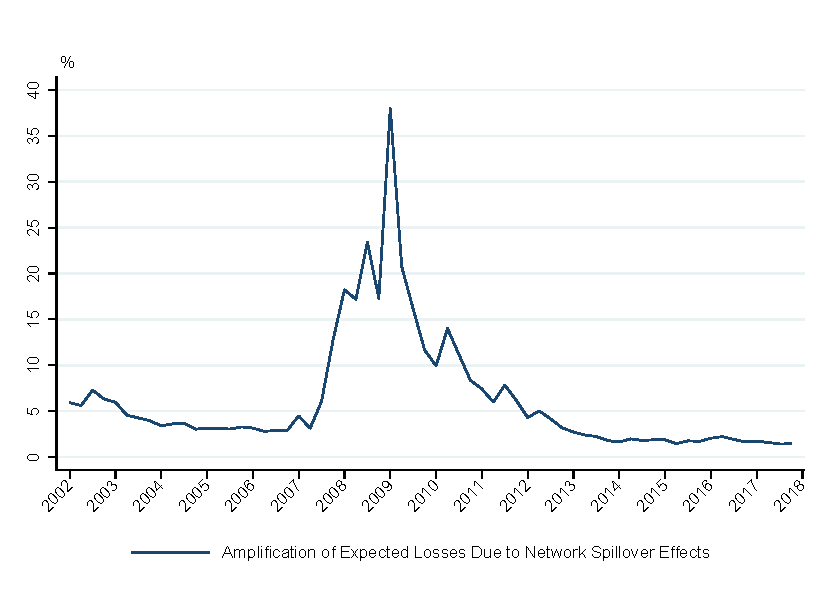
\includegraphics[width = \textwidth]{../output/NVI_benchmark.pdf}
\end{center}
\caption[]{\textbf{Network Vulnerability Index (NVI).} The NVI is an upper bound on expected losses due to default network spillovers in the U.S. financial system, expressed as a share of initial (exogenous) losses to assets outside the network. Between 2008 and 2012, network default network spillovers amplified expected losses by between 5 and 25 percent.} \label{fig:NVI_benchmark}
\end{figure}

The NVI was essentially zero from 2002-Q1 to 2007-Q4, with only a slight increase in 2007-Q3 and 2007-Q4, which immediately implies that expected vulnerability to network default spillovers were negligible for this period. Contrary to some narratives of the crisis, we do not observe any substantial buildup of network fragility of the kind we study in the years leading up to the crisis. To understand this result, we decompose our spillover measure into two factors: the weighted average of probabilities of default ($\frac{\Sigma \delta_i c_i}{\Sigma c_i}$) and a `connectivity multiplier' ($\frac{1}{1-\beta^+}$) that captures the magnitude with which initial losses in outside assets can be transmitted and amplified through network connections. The final NVI measure is the product of these two components. 

As Figure \ref{fig:NVI_components} shows, both factors contribute to the low spillover measure in the period 2002-Q1 to 2007-Q4. Because probabilities of default were miniscule in this period, the weighted average default probabilities were close to zero. Since Moody's EDF  probabilities are physical, they are adjusted for risk and thus unlikely to arise because of any low risk premium observed during this period\footnote{In addition, version 9 of KMV generally adjusts probabilities of default (upwards) for this period taking into account the ex-post defaults observed during the crisis that were not expected before it, minimizing the concern that our results are driven by any potential underestimation of default probabilities before the crisis.}. Over the same period, the connectivity multiplier declined by 10 percent. Thus, neither the vulernability of firms to default nor the inner topology of the financial network signaled any increased vulnerability.

\begin{figure}[h!]
\begin{center}
\includegraphics[width = \textwidth]{../output/NVI_components.pdf}
\end{center}
\caption[]{\textbf{NVI Decomposition.} The NVI is the product of the asset-weighted probability of default of firms inside the network and a ``connectivity multiplier'' that captures the degree of amplification and transmission created by defaults inside the network..} \label{fig:NVI_components}
\end{figure}

During the height of the crisis, between 2008-Q1 and 2008-Q4, outside assets (especially real estate) experienced sharp declines in realized and future expected values, pushing up our measure of spillovers. The connectivity multiplier, in contrast, was a mitigating factor, as it noticeably declined, reflecting financial institutions’ desire to reduce their counterparty exposure to each other in times of stress. In fact, the decline in the connectivity multiplier over 2008 was as large as the decline observed over the six preceding years 2002-2007. Figure \ref{fig:betas} shows $\beta^+$, the maximum liability connectivity selected at each point of the sample, which drives this dynamic. Overall, in late 2008 the increase in default probabilities outweighed any mitigation from lower connectivity. Our estimates indicate that expected network default spillovers over this period could amplify total initial losses by at most 11.4 percent. Whether 11.4 percent should be considered a small or large number is in the eye of the beholder.

\begin{figure}[h!]
\begin{center}
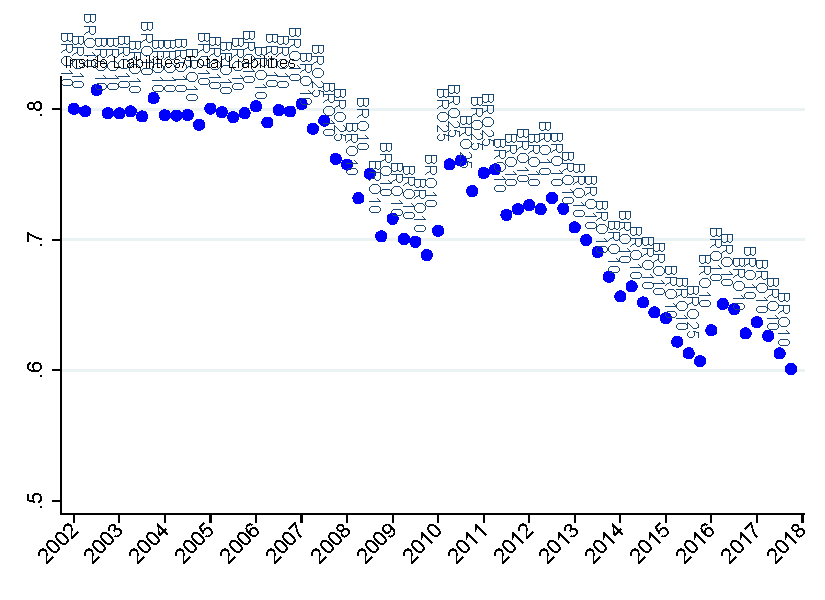
\includegraphics[width = \textwidth]{../output/connectivities_1.pdf}
\end{center}
\caption[]{\textbf{Maximum Liability Connectivity Among Large BHCs ($\beta^+$)}. The most interconnected BHC before the financial crisis was JP Morgan \& Chase. After Goldman Sachs and Morgan Stanley join the BHC sample in 2009, they become the most interconnected firms for the remainder of the sample.} \label{fig:betas}
\end{figure}

In 2009-Q1, after the failure of several financial institutions and with the crisis now global in scope, the spillover measure jumped markedly, with our estimates indicating that expected network default spillovers over this period could amplify total initial losses by up to 25 percent, the largest value observed in our sample. The large increase from 2008-Q4 to 2009-Q1 was driven by both default probabilites and financial connectivity. Expected losses increased not only because real estate kept deteriorating, but also because the slowdown in real economic activity induced an increase in expected losses for almost all categories of outside assets, including commercial, industrial and consumer loans. Financial connectivity also increased, driven by the failure of some network nodes and the merger and consolidation of various other nodes. Keeping in mind that our estimates are always upper bounds and not point forecasts, to the best of our knowledge, a 25 percent amplification is the largest empirical estimate for network spillovers in the literature. Estimates that exceed 25 percent in the literature usually rely on additional amplification mechanisms (like bankruptcy costs -- see Section \ref{sec:robustness} -- or the interaction of default cascades with other phenomena, such as runs and fire-sales. The NVI remains highly elevated in 2009-Q2 at 23 percent before dropping to 18.6 percent and 12.5 percent in 2009-Q3 and 2009-Q4, respectively.

After 2009, our spillover measure hovered between 5 and 10 percent until 2012, when the European crisis started to recede. From 2013 onward, the measure steadily decreased and reached pre-crisis levels by 2015. The most important contributor to this decrease was the reduction in the probability of default of financial institutions, particularly bank holding companies that strengthened their equity capital positions substantially over this period. Financial connectivity remained elevated until 2014 and has been declining ever since. Starting in 2015, average default probabilities have slightly increased. However, because financial connectivity has continued to decline between 2015 and 2017, our overall measure of spillovers is little changed.

\subsection{Results of FR-Y9C Asset and Liability Line-Item Classifications}

Tables \ref{tab:perc_assets} and \ref{tab:perc_liabs} show what percentage of BHC inside and outside assets and liabilities are attributable to each of several broad categories of balance sheet items, based on our classifications in Tables \ref{tab:assets_y9c} and \ref{tab:liabilities_y9c}.

These being BHCs, it is unsurprising that deposits comprise a large portion of both inside and outside liabilities. Inside assets are mostly comprised of repurchase agreements, federal funds, and deposits, while outside assets are mostly loans and mortgage-backed securities.

\newpage

\begin{table} [H]\centering
\def\sym#1{\ifmmode^{#1}\else\(^{#1}\)\fi}
\begin{minipage}{.48\textwidth}
\input{../output/asset_in_formatted}
\end{minipage}%
\begin{minipage}{.48\textwidth}
\input{../output/asset_out_formatted}
\end{minipage}
\centering
\caption[]{\textbf{Shares of BHC Assets Inside and Outside the Financial System By Category, 2016-Q4.}} \label{tab:perc_assets}
\end{table}

\newpage

\begin{table} [H]\centering
\def\sym#1{\ifmmode^{#1}\else\(^{#1}\)\fi}
\begin{minipage}{.48\textwidth}
\input{../output/liab_in_formatted}
\end{minipage}%
\begin{minipage}{.48\textwidth}
\input{../output/liab_out_formatted}
\end{minipage}
\caption[]{\textbf{Shares of BHC Liabilities Inside and Outside Financial System by Category, 2016-Q4.}} \label{tab:perc_liabs}
\end{table}

\subsection{Sector-Specific Average Default Probabilities}

As we discuss in Section \ref{subsec:non_bhc}, we calculate an asset-weighted average default probability for several different groupings of firms as proxies for the actual average EDF measure of their entire respective financial subsectors, so that the assets of firms in those subsectors can be incorporated into the final NVI. Figure \ref{fig:delta_externals} shows the final series for these average default frequencies at each point in our quarterly sample. For ease of comparison, we also plot an analagous average default probability (again asset-weighted) for the portion of our sample included in the FR-Y9C report. Figure \ref{fig:delta_externals} shows that the default probabilities for each subsector exhibit similar movements. All sectors show greatly heightened default probabilities during the financial crisis, with the average default probabilities of broker dealers and the `other' category elevating earliest in the crisis and remaining heightened for the longest. The largest default probability magnitudes come from the `other' category, and from real estate investment trusts, which experienced a number of defaults around this time\footnote{To see the firms whose default probabilities are included in each sector subsample at a snapshot of our data sample (2016-Q4), as well as the asset-weights assigned to them, see Tables \ref{tab:sample_dealers}, \ref{tab:sample_insurance}, \ref{tab:sample_reit}, and \ref{tab:sample_other}.}. 

\begin{figure}[h!]
\begin{center}
\includegraphics[width = \textwidth]{../output/delta_externals.pdf} 
\end{center}
\caption[]{\textbf{Sector-Wide Asset-Weighted Average Probabilities of Default.} Using firm-specific EDF measures and total firm assets, we calculate asset-weighted average expected default frequencies for each financial subsector in the estimated network at each quarter in our sample. These probabilities are used in our final network vulnerability measure to fill in portions of the financial sector not covered by the FR-Y9C. All sectors show greatly heightened default probabilities during the financial crisis.} \label{fig:delta_externals}
\end{figure}


\subsection{Firm-Specific Contagion Indices}

A useful understanding of our NVI measure can come from investigating the NVI's variables of interest for some of the largest firms in our sample. Figure \ref{fig:info_large_contagions} plots several important firm-specific variables that contribute to the NVI for four large BHCs - JP Morgan \& Chase, Wells Fargo, Bank of America, and Citigroup. Measures that feed directly into the NVI - outside assets $c$ and connectivity $\beta$ - are plotted alongside the contagion index measure defined in \Cref{sec:model}. 

\begin{figure}[h!]
\begin{center}
\includegraphics[width = \textwidth]{../output/info_large_contagions.pdf}
\end{center}
\caption[]{\textbf{Firm-Specific Variables for Select Large BHCs.} The figures show the net worth (the difference between total liabilities and total assets), total assets outside the financial system, the ratio of inside liabilities to total liabilites (connectivity), and the contagion index for several large BHCs.} \label{fig:info_large_contagions}
\end{figure}

Figure \ref{fig:info_large_contagions} shows how the general, system-wide dynamics described above play out for a few important financial institutions. The path of financial connectivity for these firms differs from 2002-2008, but falls or remains steady for each of them either during the financial crisis or soon thereafter. Financial connectivity for each of these large firms had risen back to pre-crisis levels by the end of 2016.

Three of these four firms were parties to large-scale acquisitions of other financial firms at the time of the crisis (Bear Stears for JPM, Merrill Lynch for BAC, and Wachovia for WFC), which caused their outside assets (and assets generally) to increase around that time. Naturally, this causes increases in the `contagion index', which is linked to the probability of a failure by that firm causing subsequent contagion defaults. As the smallest of these four firms' contagion index is larger than any one of their net worths, we cannot rule out the possbility that a large exogenous shock to one firms' assets could cause a contagion failure in another of these four firms. However, given the large size of each of these firms' outside assets compared to each other's contagion indices, we know that the probability of a shock to one firm's assets causing default in any other of these firms must be lower than the probability of that firm defaulting because of its own exogenous shock (see 
\citet{glasserman2015likely}. Table \ref{tab:large_instit} shows the same field values for 19 of the largest BHCs in the sample for the final period of our data, 2016-Q4.

\newpage

\begin{landscape}
\begin{table}[htbp]\centering
\def\sym#1{\ifmmode^{#1}\else\(^{#1}\)\fi}
\input{../output/large_instit_breakdowns_clean}
\caption[]{\textbf{Select Firm-Specific Variables for Large BHCs, 2016-Q4}. The table shows the net worth (the difference between total liabilities and total assets), total assets outside the financial system, the ratio of inside liabilities to total liabilites (connectivity), and the contagion index for BHCs in the last period of our sample.}\label{tab:large_instit}
\end{table}
\end{landscape}
\newpage

\begin{figure}[h!]
\begin{center}
\includegraphics[width = \textwidth]{../output/NVI_contributions.pdf}
\end{center}
\caption[]{\textbf{Additive Contributions to NVI by Sector.} The contribution of each sector to the NVI is that sector's average default probability, weighted by the portion of system-wide outside assets belonging to the individual sector, and multiplied by the connectivity component of Figure \ref{fig:NVI_components}. The `Other' category consistently contributes the largest magnitude of any sector, followed by bank holding companies. Real estate investment trusts, due to their relatively low quantity of outside assets, contribute the least. The final NVI measure is the sum of each sector's contribution.} \label{fig:NVI_contributions}
\end{figure}

\begin{figure}[h!]
\begin{center}
\includegraphics[width = \textwidth]{../output/beta_dist.pdf}
\end{center}
\caption[]{\textbf{Distribution of Liability Connectivities.} The figure shows distribution statistics for $\beta$, the balance sheet estimated portion of firm liabilities held by other financial firms, for bank holding companies in each quarter of our sample. The value $\beta^+$ refers to the high $\beta$ chosen for ther purposes of calculating the financial connectivity multiplier in the benchmark NVI.} \label{fig:beta_dist}
\end{figure}